\section[Weyl and Dirac cones]{Weyl and Dirac cones in condensed matter physics}
\label{sec:weyl-dirac-cones}
%% Much is taken from https://www.tandfonline.com/doi/pdf/10.1080/00018732.2014.927109?needAccess=true
Dirac and Weyl cones are the emergence of non-gapped linear energy bands in condensed matter physics, in effect exhibiting relativistic behavior at non-relativistic speeds.
We here give a brief introduction to these materials.
The system and its relation to high energy physics is discussed first.
Then, several perturbations of the system are introduced.
The topological nature of the system is considered in the context of Chern numbers and Berry curvature.
Lastly, we go into tilted Dirac cones in some more depth.
The reader is also advised to consult the many recent reviews on the topic, notably~\textcite{armitageWeylDiracSemimetals2018} for a general introduction and overview of the field,~\textcite{jiaWeylSemimetalsFermi2016} with a focus on material realizations, and~\textcite{chernodubThermalTransportGeometry2021} which is the most directly relevant for our work, discussing in particular thermal transport and the analogy to high energy physics.

% Firstly, we will consider the so-called band crossing, and how the opening of a gap at the band crossing behaves differently in two and three dimensions.
% Then, various perturbations that do not open a gap will be considered, giving interesting effects in the dispersion relations.
% Lastly, a consideration of these materials in light of Berry curvature and the topological quantity of Chern numbers will be given.

The standard model for metals in condensed matter physics is the Landau Fermi liquid~\cites{landauTheoryFermiLiquid1956,chernodubThermalTransportGeometry2021}, where electrons are described by the Hamiltonian \( p^2 /2 m^* \), with \( m^* \) some effective mass.
The model works remarkably well for many systems, but fails for Dirac materials, where the electrons behave as ``Dirac fermions''.
The notion of a ``Dirac fermion'' is almost comical from a high energy point of view~\cites{chernodubThermalTransportGeometry2021,vozmedianoTheoreticalPhysicsColloquium2021} -- what else can they be?
A fermion is by its very definition a Dirac spinor.
In condensed matter language, however, we mean by fermion that it obeys the Pauli exclusion principle and follows the Fermi-Dirac distribution.
By Dirac fermion in condensed matter we mean fermions whose effective low-energy Hamiltonian is linear in momenta, they obey an effective Dirac equation.

This field unifies concepts from high and low energy physics;
a ``new era of grand unification of low and high energy physics'' as~\textcite{chernodubThermalTransportGeometry2021} puts it.
The emergent Dirac and Weyl cones in condensed matter physics follow in beautiful analogy their high energy counterparts.
Thus, the theory and results from high energy physics may be applied in these emergent Dirac systems.
Likewise, these materials offer the opportunity to probe the fundamental theories of our universe, and beyond, at much lower energy and cost scales.
% Unfortunately, some concepts of \gls{qft} and high energy physics are somewhat inaccessible for condensed matter physicists.
Unfortunately, the language of \gls{qft} and high energy physics is somewhat inaccessible for condensed matter physicists.
At the same time, the condensed matter descriptions have been difficult to relate back to the \gls{qft} formalism.
So while the intersection of the two fields offers the possibility of great new insight, it also comes with some misunderstandings.
Some phenomena are known under different names, while different phenomena may be mistaken for the same.
The recent and excellent review paper by~\textcite{chernodubThermalTransportGeometry2021} attempts to make the topics approachable for researchers from both fields, with its ``main purpose \dots to present the basic notions underlying new developments in condensed matter in a language equally accessible to both high energy and condensed matter communities''.

We wish here to briefly illuminate the connection between the high energy Dirac theory and the Dirac and Weyl semimetals of condensed matter physics, assuming the reader to be an expert in neither.
The (massive) Dirac equation reads
\begin{equation}
  (i \slashed{\partial} - m ) \psi = 0,
\end{equation}
where \( \slashed{\partial} = \gamma^{\mu} \partial_{\mu} \), \( \gamma^{\mu} \) are the so-called \emph{gamma matrices},%
\footnote{Also known as the Dirac matrices. They are any irreducible matrix representation of the Clifford algebra.}
\( m \) is some mass parameter, and \( \psi \) the Dirac spinor.
Note also that natural units \( c = \hbar = 1 \), as usual, is used and that the systems is \( 4\times 4 \).
It may of course be written as a Schrödinger equation~\cite{chernodubThermalTransportGeometry2021} \( i \partial_t \psi = H \psi \), with \( H = \gamma^0 m + \gamma^0\gamma^ip_i \).
The great insight of Dirac was that due to the requirement of Lorentz invariance, the momentum and time operators had to appear at the same order, as opposed to the standard free particle \( H = p^2 /2m \).
% The great insight of Dirac, was that the momentum and time operators had to appear at the same order, due to the requirement of Lorentz invariance.
Shortly after Dirac published his theory, Weyl commented that for a massless particle, the equation could be decomposed into two \( 2 \times 2 \) equations -- a Weyl decomposition.
This yields two independent subsystems, themselves also linear in momentum,
\begin{equation}
  \label{eq:156}
  H_{\pm} = \pm \vec{\sigma} \cdot \vec{p},
\end{equation}
with the \( \pm \) defining the \emph{chirality}%
\footnote{For massless particles equivalent to the helicity.}
of the Weyl component.

Interestingly, massless Dirac fermions may appear in condensed matter as low energy effective descriptions of electronic systems near a two-band crossing.
Instead of obeying the Landau Fermi liquid theory, like most materials, they obey a Dirac equation, with the speed of light being replaced by the Fermi velocity $v_F$.
As in the high energy case, the Dirac equation may be decomposed into chiral Weyl equations
\begin{equation}
  \label{eq:3}
H_D = s v_{F} \vec{\sigma} \vec{p},
\end{equation}
where $\vec{\sigma}$ are the Pauli matrices, $v_F$ the Fermi velocity, $\vec{p}$ the momentum, and $s=\pm 1$ denotes the chirality.
% It is here important to note that the spin degree of freedom expressed by the Pauli matricies, may either be real spin or some pseudo spin degree of freedom.
It is here important to note that the Pauli matrices represent either real spin degree of freedom or some pseudo spin degree of freedom.
Examples of pseudo spin are that of bipartite lattices, such as graphene, in which case one must be careful when for example applying time-reversal, as only real spin is odd under this operation, and not pseudo spin.

These linear low energy emergent systems may appear in both 2D and 3D.
There are, however, important differences depending on the dimensionality.
When we here refer to Dirac and Weyl materials, we always mean 3D systems.
% , which have become the norm in the literature.
% In some older literature, the term might also be applied to 2D systems, such as graphene.

\label{sec:stability-of-gap}
The dispersion of the Hamiltonian \eqref{eq:3} has a band crossing at  $\vec{p} = 0$.
For the two-dimensional case, a perturbation on the form $m \sigma_z$, with $m$ some parameter, opens a gap in the dispersion.
This is easily verified by writing out the Hamiltonian and solving the eigenproblem
\begin{align}
  H_D^{(2D)} &= s v_{F} (p_x \sigma_x + p_y \sigma_y) + m \sigma_z,\\
  \left|
  H_D^{(2D)} - E
  \right| &= 0.
\end{align}
As the Hamiltonian commutes with the momentum operator, we replace the momentum operator with its eigenvalues
\begin{equation}
E_{\pm} = \pm v_F \hbar \sqrt{k_x^2 + k_y^2 + \frac{m^2}{\hbar ^2 v_{F}^2}}.
\end{equation}
For a non-zero \( m \), there are no solutions $k_x, k_y$ making the energy levels degenerate (i.e. \( E_{\pm} = 0 \)).
The crossing is thus only protected by symmetry considerations, and is not \emph{topologically protected}.
\todo{Is this usage of topologically protected correct?}


In three dimensions the situation is somewhat different, with the Hamiltonian  
\begin{equation}
  H_D^{(3D)} = s v_F ( p_x \sigma_x + p_y \sigma_y + p_z \sigma_z).
\end{equation}
In this case, no perturbing term may open a gap at the crossing.
There is no $2\times 2$ matrix $\sigma_4$ that anticommutes with the Pauli matrices and while also being linearly independent, i.e. there is no ``fourth'' Pauli matrix;
therefore no perturbative term will open the gap.
Say for example we add a term like $m \sigma_z$, where the $z$-direction was chosen arbitrarily.
The only effect this will have on the crossing is to translate it in $k_z$.
Tying this back to the accidental degeneracy of \cref{sec:accidental-degeneracy}, we see that no matter the perturbation, the three-dimensional momentum space will always have a point of degeneracy, i.e., a crossing.
The crossing is \emph{topologically protected}.
A more formal approach to topological materials is that of topological invariants -- numbers related to the topology of the material.
Having a non-trivial topological invariant number is the very definition of topological materials, and we will in \cref{sec:chern-number-weyl} show that Dirac cones make the Chern number of these materials non-trivial.

\subsubsection{Lorentz breaking perturbations}
As opposed to high energy physics, the emergent Dirac equation in condensed matter physics need of course not be Lorentz invariant.
We may therefore introduce terms that break Lorentz invariance.
Introduce to the system a pseudospin degree of freedom, thus extending the system to $4\times 4$-matricies;
in effect re-constructing the full Dirac equation from the Weyl equations, and then introduce perturbations.
The Hamiltonian of the system
\begin{equation}
  \label{eq:5}
  H = v_F \tau _x \otimes \vec{\sigma} \vec{p} + m \tau _z \otimes I_2 + b I_2 \otimes \sigma _z + b' \tau _z \otimes \sigma _x,
\end{equation}
with $\vec{\tau}$ the Pauli matrices related to the pseudospin, and $I_2$ the identity matrix of dimension 2.
The perturbing parameters $m, b, b'$ are a mass parameter, and Zeeman fields in the $z$ and $x$ direction, respectively~\cite{armitageWeylDiracSemimetals2018}.
Ignore for now $b'$, i.e. $b' = 0$, which is related to a state known as the line node semimetal.
Notice that the $b$ term breaks time-reversal symmetry in the system, as the real spin $\sigma $ is odd under time-reversal.
The eigenvalues of this system~\cite{armitageWeylDiracSemimetals2018}
\begin{equation}
  E_{s \mu }(\vec{k}) = s \left[
    m^2 + b^2 + v_{F}^2k^2 + 2 \mu  b \sqrt{v_F^2 k_z^2 + m^2}
  \right]^{\frac{1}{2}},
\end{equation}
with $s=\pm 1, \mu = \pm 1$ encoding the degeneracies related to the spin and pseudospin degrees of freedom, respectively.
There are still linear dispersions for $b > m$.
For $b < m$, a gap opens, and the dispersion is non-linear.
In fact, for \( b > m \), the perturbation is simply a shift in $k_z$ of the Dirac cone, similar to what was discussed in the \( 2\times 2 \) case, as  is seen by rewriting
\begin{equation}
  E_{s \mu }(\vec{k}) = s v_F
  \left[
    k_x^2 + k_y^2 + \left( \sqrt{k_z^2 +  \frac{m^2}{v_{F}^2}} + \mu \frac{b}{v_{F}} \right)^2
  \right]^{\frac{1}{2}}.
\end{equation}
This still has Weyl node solutions at $k_z^2 = (b^2-m^2) /v_F^2$, where the dispersion is linear in the vicinity of the nodal solutions.
The effect is thus to separate the two Dirac nodes in momentum space, giving a \emph{Weyl} semimetal.
This also illustrates that the decomposition in \cref{eq:3} is valid around either of the shifted nodes.
Expanding around one of the Dirac points of the Weyl semimetal, the Hamiltonian is exactly \cref{eq:3}, after decomposing the $4 \times 4$ Hamiltonian into its two chiral  $2\times 2$ Weyl constituents.
If one instead perturbs the system with a Zeeman field in the $x$-direction, $b' \neq 0$, the separation is instead in energy, giving a nodal loop where the two cones intersect.
We will not go into any depth on these types of materials.

The three cases described here: unperturbed, where the two cones are superimposed; perturbed by $b$, where the cones are separated in momentum; and perturbed by $b'$, where the cones are separated in energy, are shown in \cref{fig:conetypes}.
Notice that in the two latter cases, the Dirac points, i.e. crossings, are not superimposed.
As will be substantiated more in \cref{sec:chern-number-weyl}, this makes the crossings very robust, as the two nodes must merge before a gap may be opened.


The Hamiltonian in \cref{eq:3} is not the most general \( 2 \times 2 \) Weyl system if we allow for anisotropy in the system.
In three dimensions we have more generally the \emph{tilted} Weyl Hamiltonian
\begin{equation}
  \label{eq:4}
  H_s = (\vec{t}^{s} + s \vec{\sigma}) (\vec{v} \odot \vec{p}),
\end{equation}
where $\vec{t}^{s}$ is  the \emph{tilt vector}, $\vec{v}$ is some anisotropic velocity, $(\vec{v} \odot \vec{p})_i = v_i p_i$ is the Hadamard product of the anisotropic velocity and the momentum,  and $\vec{\sigma}$ are the Pauli matrices corresponding to spin degree of freedom.
By a simple rescaling of the momenta, we may in general consider a system with isotropic Fermi velocity \( v_F \), giving
\begin{equation}
  \label{eq:hamil-tilt-isotropic}
  H_s = s v_F \vec{\sigma} \vec{p} + v_F \vec{t}^s \vec{p}.
\end{equation}
The energy bands are
\begin{equation}
  \label{eq:tilted-eigenvalue}
  E_s(\vec{k}) = \pm v_F |k| + v_F \vec{t}^{s} \vec{k},
\end{equation}
as shown in \cref{fig:tilted-cones}.
These types of systems, which are the systems of interest for this thesis, are considered in detail in \cref{sec:typeii}.

\begin{figure}[p!]
  \centering
  % \includegraphics[width=\textwidth]{figures/cone}
  % \includegraphics[width=\textwidth]{figures/cones_types-verysmall}
  \iftoggle{full-size-image}{%
    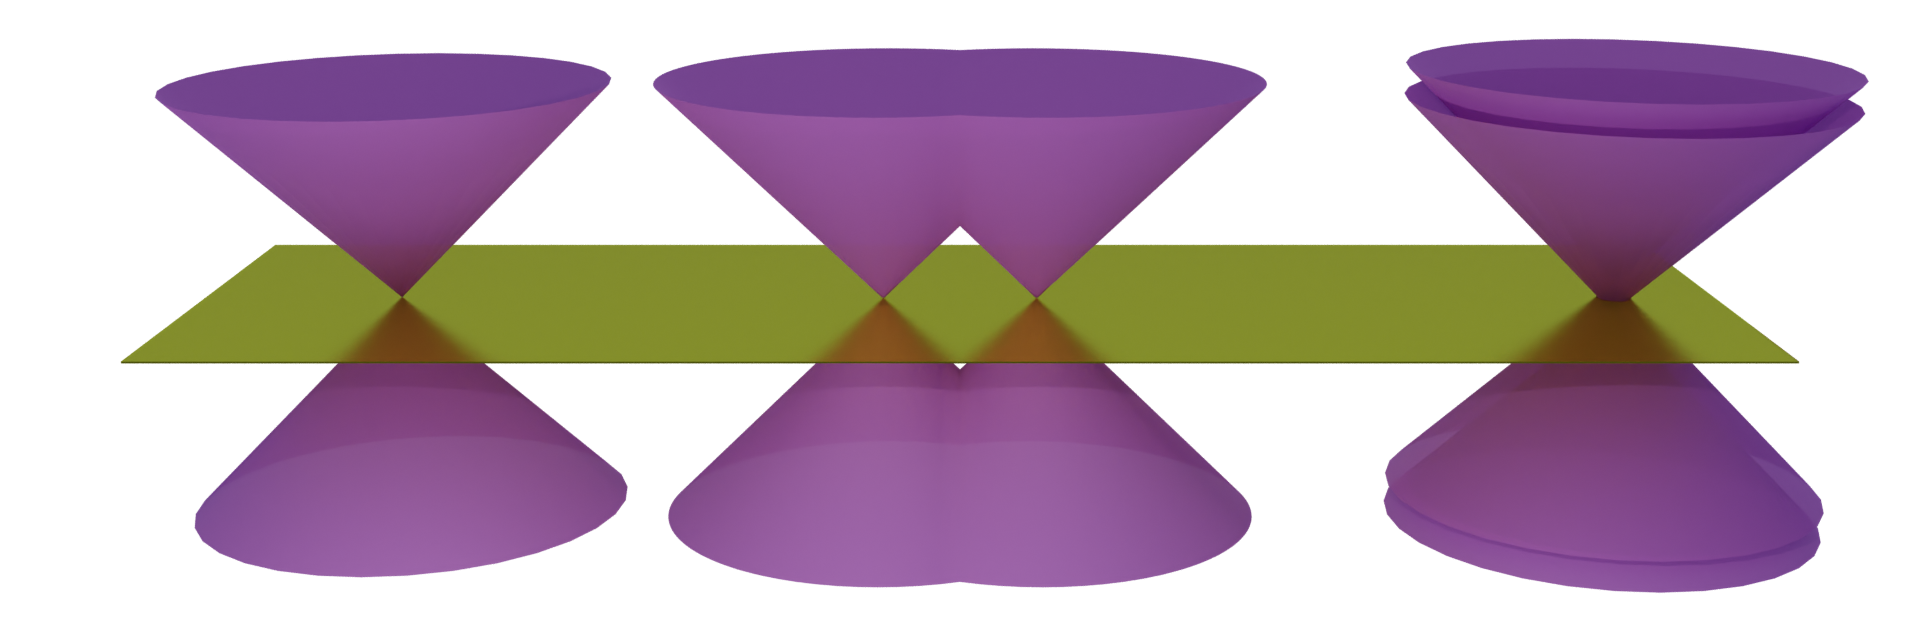
\includegraphics[width=\textwidth]{figures/cones-types-col1-opaque}
  }{%
    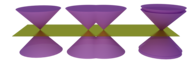
\includegraphics[width=\textwidth]{figures/cones-types-col1-opaque-small}
  }
  \caption{%
    % Dirac cones in the $k_z, k_x$-plane, .
    Dirac cones in the plane, with the perpendicular momentum set to zero.
    \textbf{(Left)} Dirac material with superimposed cones. \textbf{(Center)} Time-reversal symmetry broken, giving a Weyl material with the cones separated in momentum  space. \textbf{(Right)} The cones shifted in energy, giving a nodal loop.
    \todo{Consider making middle one with mass term.}
  }
  \label{fig:conetypes}
\end{figure}

\begin{figure}[p!]
  \centering
  % \includegraphics[width=0.75\textwidth]{figures/tilt_cone}
  % \includegraphics[width=0.75\textwidth]{figures/conesTransparent-verysmall.png}
  % 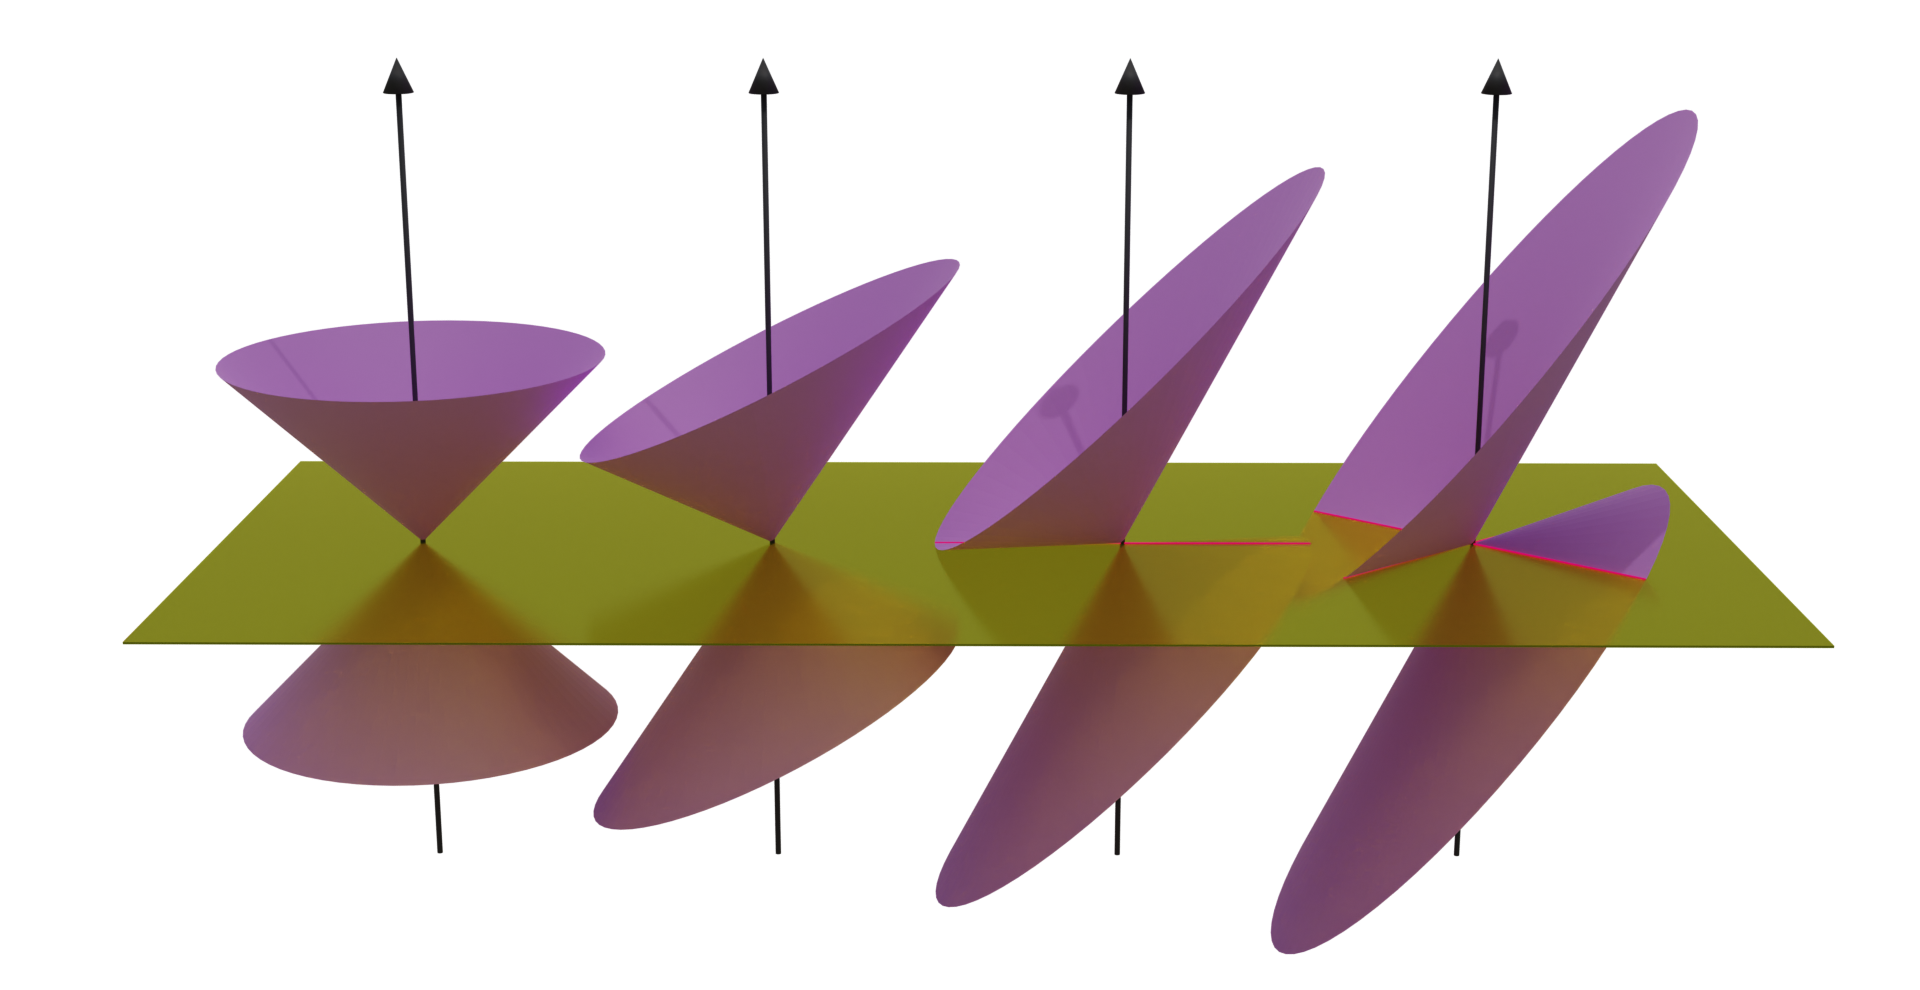
\includegraphics[width=\textwidth]{figures/cones-tilt-color1.png}
  \iftoggle{full-size-image}{%
    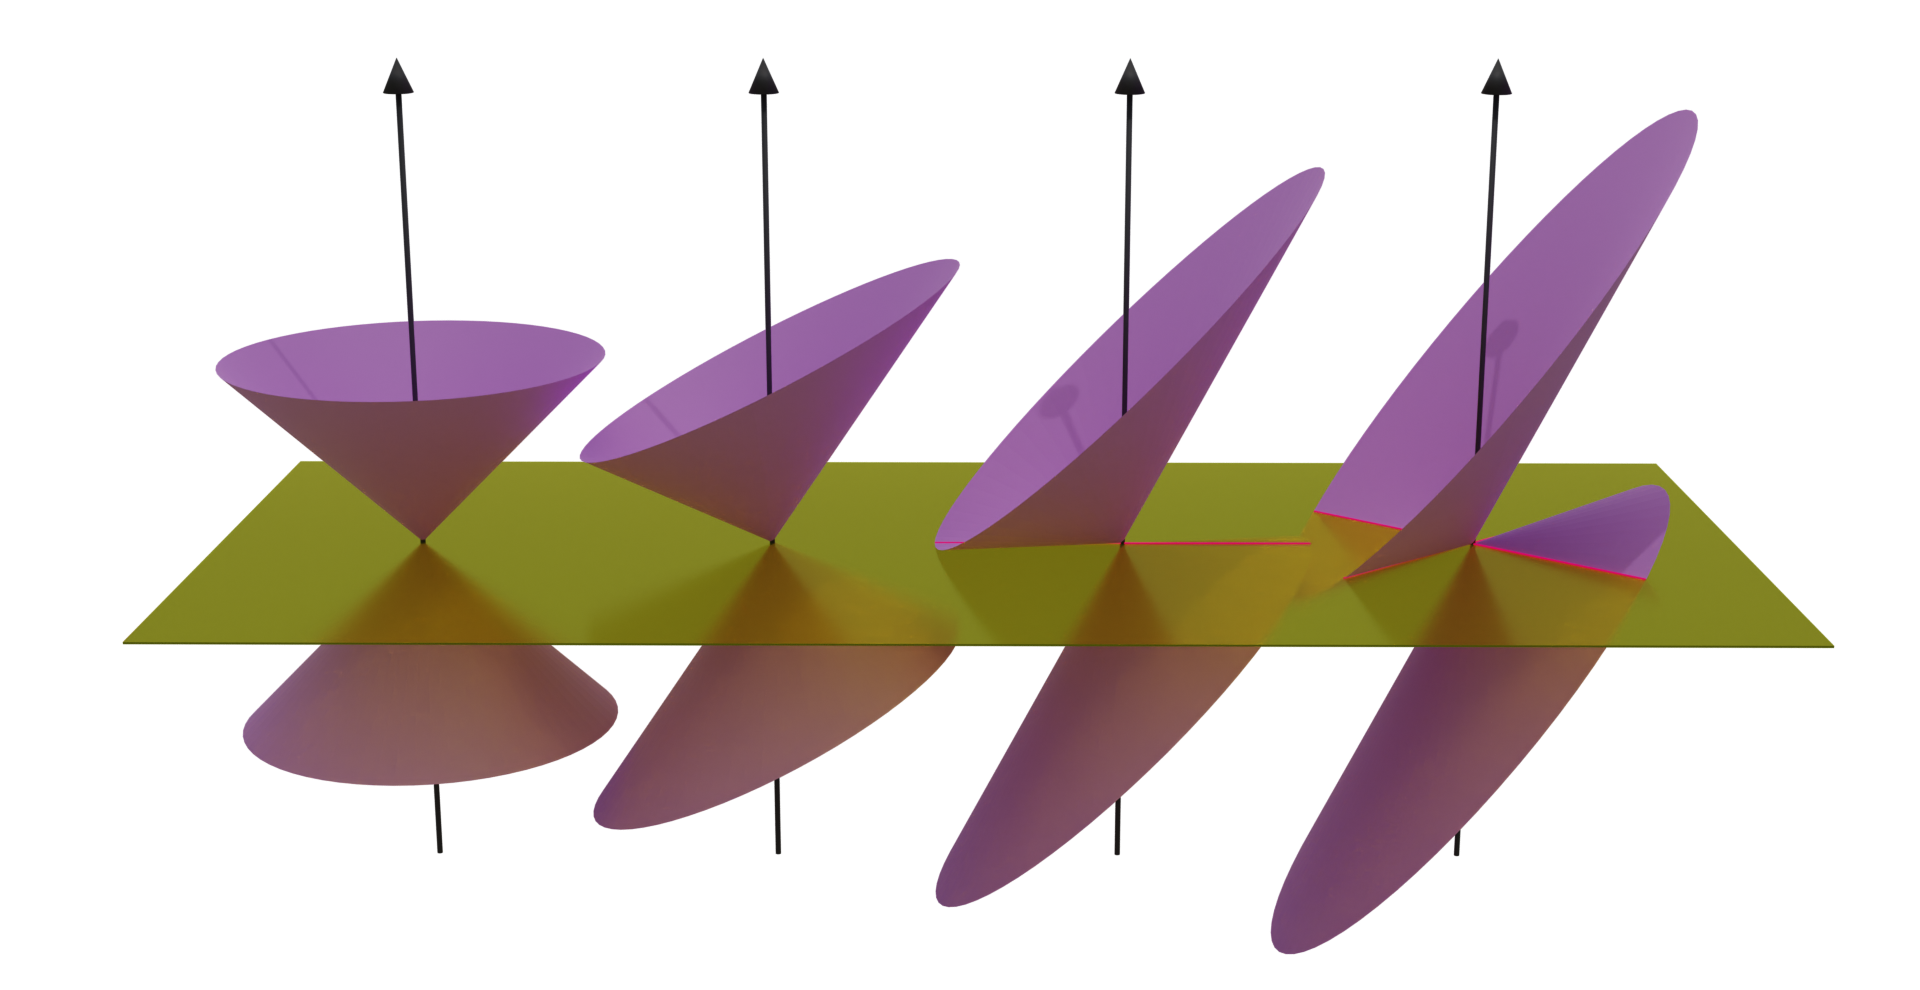
\includegraphics[width=\textwidth]{figures/cones-tilt-color1}
  }{%
    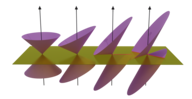
\includegraphics[width=\textwidth]{figures/cones-tilt-color1-small}
  }
  \caption{Tilted Dirac cones in the plane, with the perpendicular momentum set to zero.
    From left to right the tilt increases, from no tilt in the first cone to overtilt in the last.
    The three first are Type-I Weyl semimetals, the last is a Type-II semimetal.
    The Fermi surface is marked in red.
    See main text for details.
    \label{fig:tilted-cones}
  }
  % \caption{Tilted cone. \textbf{(Left)} Type I Weyl semimetal, with no tilt.
  %   \textbf{(Center)} Type  I Weyl semimetal, with tilt.
  %   \textbf{(Right)} Type II Weyl semimetal, meaning the tilt makes the upper part of the cone go below horizontal.}
\end{figure}

\subsection{Chern number of the Weyl point}\label{sec:chern-number-weyl}
In order to more explicitly demonstrate the topological nature of the tilted Weyl cone in \cref{eq:3}, we will find a non-zero topological invariant associated with that state.
Thereby showing that the material is topological.
The topological number we will calculate is the Chern number, related to the Berry curvature of the bands in some enclosed surface.
In order to calculate the Chern number, we must first find an expression for the Berry curvature of our system.
This derivation will follow closely Berry's original derivation~\cite{berryQuantalPhaseFactors1984} of the Berry phase of a two-level system with the Hamiltonian
\begin{equation}
  \label{eq:6}
  H(\vec{R}) = \frac12 \vec\sigma \vec{R}.
\end{equation}
Some notation has been modernized with inspiration from the treatment of the Berry phase of the spin-$1 /2$ particle in an external magnetic field in~\textcite{holsteinAdiabaticTheoremBerry1989}.

Suppose we have a Hamiltonian $H(t)$, and that its $t$-dependence can be parameterized by $\vec{R} = \vec{R}(t)$, as in $H(t) = H(\vec{R}(t))$.
Any evolution of the Hamiltonian through time, may then be described as a geometric path through the $\vec{R}$-space.
As the reader might be aware, Berry's most famous discovery was that a closed path through $\vec{R}$-space gives an observable phase to the system, unlike the non-physical dynamical phase, which may be removed by a suitable choice of gauge.
Here we will however focus on the so-called Berry curvature, $\vec{B}$, a vector field that will be shown to be useful in the categorization of topological materials.
Note that there is some variation in the literature on the naming of the various quantities, and the sign convention used.
In particular, the term \emph{Berry curvature} will in some literature refer to a rank two tensor;
what we call Berry curvature is referred to as the \emph{Berry field strength}.
In particular, if we let the rank two tensor be denoted $F_{ij}$, the Berry curvature is given by
\begin{equation}
  B_i = \epsilon_{ijk} F_{jk}.
\end{equation}

The Berry curvature for the state $n$ is explicitly defined as~\cite{berryQuantalPhaseFactors1984}
\todo{Should we add some more comments about adabiatic? See topo book}
\begin{equation}
  \vec{B_n}(\vec{R}) =
  -\Im \sum_{m\neq n}
  \frac{
    \braket{n(\vec{R}) | \vec{\nabla}_{\vec{R}} H | m(\vec{R}) }
    \times
    \braket{m(\vec{R}) | \vec{\nabla}_{\vec{R}} H | n(\vec{R}) }
  }{
    (E_m(\vec{R}) - E_n(\vec{R}))^2
  },
\end{equation}
where $\times $ denotes the cross product.
Notice that for a degeneracy $E_n = E_m$ there will be a pole in $\vec{B_n}$.
Considering the Berry curvature as a field in $\vec{R}$-space, this resembles a source, as will become relevant later.
This may now be applied to for example the Weyl semimetal, both in the interest of solidifying the above theory, and as it will be useful in future consideration.

The Hamiltonian around the (untilted) Weyl point is
\begin{equation}
  H = v_F \vec{\sigma} \cdot \vec{p},
\end{equation}
with $v_F$ the Fermi velocity, $\vec{\sigma}$ the Pauli matrices, and $\vec{p}$ the momentum operator.
% \todo{Now suddenly R is not dependent  on t??}
By letting $\vec{R} = v_F \vec{p}$, the Berry curvature of the Hamiltonian can be found.
The eigenvalues of this system are%
\footnote{Technically, this is sloppy notation, as the eigenvalues are of course \( E_+ = -E_- = v_F |k| \). We chose to use the above notation for clarity and to be more true to Berry's original derivation, even though that included implicit interchanging of \( \vec{k} \leftrightarrow \vec{p} \).}
\begin{equation}
    E_+ = -E_-
    = |R|.
\end{equation}
The aforementioned degeneracy is here of course the Weyl point, where $E_+ = E_- = 0$.
Noting that
\begin{equation}
  \label{eq:gradHamil}
  \nabla_{\vec{R}} H = \vec\sigma,
\end{equation}
we can calculate the Berry curvature easily.
Denote by $\ket{+}$ the state with the eigenvalue $E_+$ and $\ket{-}$ the state with the eigenvalue $E_-$.
Take also, without loss of generality, $\vec{R}$ to be in the $z$-direction.
This gives
\begin{equation}
  \vec{B}_+ = -\Im
  \frac{
    \braket{+ | \vec\sigma | -}
    \times
    \braket{- | \vec\sigma | +}
  }{
    4 R^2
  }.
\end{equation}
As $\ket{+}$ and $\ket{-}$ are eigenstates of $\sigma_z$ and orthogonal to each other, only the $z$-component of the cross product may contain non-zero contributions.
\begin{equation}
  \begin{split}
    \vec{B}_+ &= - \frac{\hat{z}}{4 R^2}
    \Im \left(
    \braket{+ | \sigma_x | -}
    \braket{- | \sigma_y | +}
    -
    \braket{+ | \sigma_y | -}
    \braket{- | \sigma_x | +}
    \right)\\
    &= - \frac{ \hat{z}}{2 \vec{R}^2}.
  \end{split}
\end{equation}
Here, the effect of the Pauli matrices on the eigenvectors was used, according to
\begin{align}
  \sigma_x \ket{\pm} &= \ket{\mp}\\
  \sigma_y \ket{\pm} &= \pm i \ket{\mp}
\end{align}
Returning to general axis orientations, one has
\begin{equation}
  B_+ = - \hat{R} / 2\vec{R}^2 = - \vec{R} / 2 \vec{R}^3.
\end{equation}
For the $\ket{+}$-band, the Weyl point thus takes the form of a negative monopole in $R$-space;
this motivates the requirement that Weyl points must always appear in pairs of opposite chirality, as the divergence of the Berry curvature must always be zero over the entire sample.

Extending the calculation to a tilted Weyl cone
\begin{equation}
  H = v_F \vec{\sigma} \cdot \vec{p} + v_F \vec{t} \cdot \vec{p},
\end{equation}
is trivial.
The energies gain a factor \( v_F \vec{t}\cdot \vec{p} = \vec{t} \cdot \vec{R}\), however, this does not change the difference between the energies of the states.
Furthermore, the gradient of the Hamiltonian, \cref{eq:gradHamil}, gains a factor
\begin{equation}
  \nabla_{\vec{R}} H = \vec\sigma + \vec{t},
\end{equation}
which does not affect the result, as \( \braket{\pm | \vec{t} | \mp} = 0 \).
Consequently, tilting does not affect the Berry curvature.

As mentioned, the Chern number is one of several numbers that is used to classify topological materials.
The Chern number is defined as
\begin{equation}
  C = \frac{1}{2\pi} \oint_{\partial C} \vec{B_+} \cdot \mathrm{d}\vec{S},
\end{equation}
where the integral is taken over the closed surface $\partial C$, enclosing the volume $C$.
Noting that the Berry curvature has the shape of a monopole source at $\vec{p} = 0$, we immediately know the value of this quantity from electromagnetism.
We will, however, carry out the computation explicitly here.
With the divergence theorem in mind, it behooves us to find the divergence of the Berry curvature.
This divergence is zero everywhere except in the monopole source, giving
\begin{equation}
  \nabla \cdot \vec{B_+} = -\frac12 \nabla \cdot \hat{R} / R^2 = -2 \pi \delta(\vec{p}),
\end{equation}
where $\delta$ is the Dirac delta distribution.
By virtue of the divergence theorem, the Chern number is then found to be
\begin{equation}\label{eq:chern}
  C = \frac{1}{2\pi} \int_C \nabla \cdot \vec{B_+} \mathrm{d} C = -1,
\end{equation}
where the property of integrals over Dirac delta distributions was used.

Note that some literature will have a Chern number differing from \cref{eq:chern} by the sign of the Fermi velocity,
\begin{equation}
  C = - \operatorname{sign}(v_F).
\end{equation}
This simply comes from the definition of the eigenstates.
We have put the sign dependence in the state, making the $E_+$ state always have positive eigenenergy.
In the literature that instead defines $E_+ = v_F |R|$ the state's energy will depend on the sign of the Fermi velocity, and as a consequence, the sign dependence will end up in the Chern number instead.

The overall divergence of Berry curvature must be zero, or equivalently, the sum of the Chern numbers must be zero.
The Hamiltonian \cref{eq:6} chosen with the opposite chirality,
\begin{equation}
  H(\vec{R}) = -\frac{1}{2} \vec{\sigma} \vec{R},
\end{equation}
has the opposite Berry curvature, and also the opposite Chern number.
Thus, Dirac cones must appear in pairs of opposite chirality, either superimposed as the Dirac semimetal case or separated in momentum space, as the Weyl semimetal.

In light of the interpretation of the Dirac point as a monopole of Berry curvature, the discussion in \cref{sec:weyl-dirac-cones}, on page \pageref{sec:stability-of-gap}, on the stability of the band crossing in two and three dimensions gets an intuitive and geometric interpretation.
In \cref{fig:curvature_plane} the Berry curvature pole is shown in $p$-space, together with a plane parallel to the $xy$-plane, which we will denote the \emph{state plane}.
In the two-dimensional case, the state is confined to the state plane, with the $z$-position of the plane given by any mass terms $m \sigma _z$.
In the three-dimensional case, the state is not confined to this plane, as the parameter $k_z$ is a free variable, or alternatively, it may be considered as the freedom to move the state plane freely, with its initial position simply shifted by any mass terms.
It is thus obvious that one may never reach the monopole in the two-dimensional case, and thus for no $\vec{k}$ is there a band crossing.
Importantly, the Berry curvature is indeed non-zero, however any closed  curve of integration will give a Chern number of zero;
the  monopole has been moved outside the dimensionality of freedom.
\begin{figure}[ht]
  \centering
  \iftoggle{full-size-image}{%
    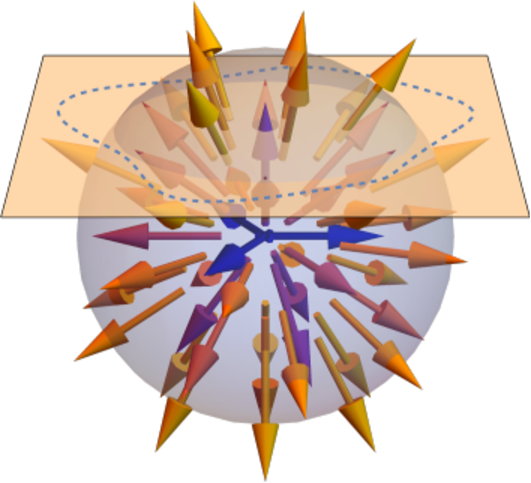
\includegraphics[width=0.5\textwidth]{figures/berryCurvePlanewpath}
  }{%
    
\includegraphics[width=0.5\textwidth]{figures/berryCurvePlanewpath-small}
  }
  \caption{The state plane, transparent yellow, parallel to the $xy$-plane and a Berry curvature monopole at the origin.
  An integration contour is shown in blue dashed.
  See main text for details.}
  \label{fig:curvature_plane}
\end{figure}


% \begin{figure}[ht]
%   \centering
%   \begin{tikzpicture}
%     \coordinate (O) (0,0,0);
%     \draw[->] (O) -- (5,0,0); 
%     \draw[->] (O) -- (0,5,0); 
%     \draw[->] (O) -- (0,0,5); 

%     \def\N{9}
%     \foreach \n in {0,...,\N}
%     {
%       \foreach \t in {0,...,\N}
%       {
%         \draw[->] (xyz spherical cs:radius=1.5,latitude={\n*360/\N},longitude={\t*360/\N}) -- (xyz spherical cs:radius=2,latitude={\n*360/\N},longitude={\t*360/\N});
%       }
%     }
%     \begin{scope}[canvas is zx plane at y=1.7,fill=red]
%       \draw[help lines, opacity=0.7] (-2,-2) grid (2,2);
%       \draw [cyan,thick] plot [smooth cycle] coordinates { (-1,0) (1,1) (1,-2) (0,-1) (-1, -1)};
%       \node[transform shape, rotate=90, yscale=2] at (-1.7,1.5) {$z = 2$}; 
%     \end{scope}
%   \end{tikzpicture}
%   \caption{todo}
% \end{figure}

\begin{comment}
%%%%   Old text, probably to be deleted %%%%%
\newpage

While the nearly free quasi-particle model performs very well for most metals, with the Hamiltonian $\frac{p^2}{2m^*}$, this models fails for the Dirac-materials.
Instead of obeying the Schrödinger equation as most materials, they obey a Dirac equation with the speed of light being replaced by the Fermi velocity $v_F$.
$$
H_D = v_F \sigma p + m v_F^2 \sigma_z.
$$
Here the spin degree of freedom $\sigma$ is either from the actual spin of the particle or some pseudo-spin degree of freedom such as a bipartite lattice.

The origin of this form for the Hamiltonian varies for different materials.
For graphene, for example, this form of the Hamiltonian follows directly from the tight binding model with a bipartite lattice.
Notice, however, that the spin degree of freedom in this case does not come from the actual spin of the particle, but is rather a pseudo spin degree of freedom coming from the effective two level system that appears as a result of the two positions in each cell.

The band structure of the Hamiltonian is easily found.
Writing out the Hamiltonian, setting $v_F=1$ for simplicity, we get
\begin{equation}
  H_D = p_x \sigma_x + p_y\sigma_y + m \sigma_z,
\end{equation}
which has eigenvalues at
$$
| H_D - E I | = 0.
$$
This gives us the solutions
\begin{equation}
  E = \pm \sqrt{
    k_x^2 + k_y^2 + m^2
  }.
\end{equation}

Just as in the particle physics case, the Dirac equation will exhibit gapless band structures as $m\rightarrow 0$.
As introducing a term $m\sigma_z$ would break inversion symmetry, such systems cannot be gapped.
One may show that in graphene, time and inversion symmetry will force the mass term to be zero, and the gap disappears.
\end{comment}
\begin{comment}
  \begin{figure}
    \begin{tikzpicture}
      \begin{axis}[
        legend style={
          at={(0.5, 0.95)},
          anchor={north},
        },
        legend cell align=left,
        width=13cm,
        cycle list name=linestyles,
        domain=-pi/2:pi/2,
        samples=201,
        ]
        \pgfplotsset{cycle list shift=-1}
        \foreach \m in {0, 0.1, 1, 2} {
          \addplot+[forget plot] {sqrt(x^2 + \m^2)};
          \addplot+ {-sqrt(x^2 + \m^2)};
          \addlegendentryexpanded{$m=\m$}
        }
      \end{axis}
    \end{tikzpicture}
    \caption{Band structure for the 2D Weyl Hamiltonian for various values of the mass term.} 
  \end{figure}
\end{comment}
